\section{Git operations}

\subsection{Add and Remove}

When you use the 'git add <file>' command, a file will be
added to the index. The file added can be a new file, or 
a file already existing in the index. When the latter is true, 
git just updates the content of that file. \par
When you add a file, it will be marked to be committed in the next
commit. 
\begin{figure}[h!] 
	\caption{Before the add}
	\centering
	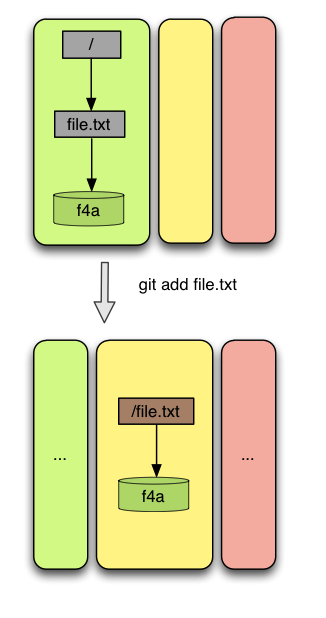
\includegraphics[scale=0.65]{images/add1.png}
\end{figure}

\begin{figure}[h!] 
	\caption{After the add}
	\centering
	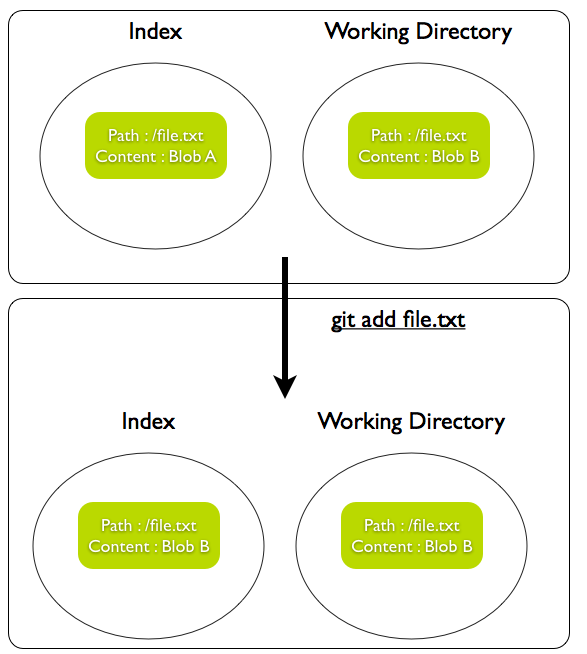
\includegraphics[scale=0.65]{images/add2.png}
\end{figure}

\pagebreak

'git rm <file>' can be seen as the inverse operation of the 'git add <file>'.
In this case Git, will remove a file from the index, so it won't appear in the
next commit. Besides being removed from index, it will also be removed from the 
working directory (if it's still there). \par
However, there are a few cases that Git prevents you from removing a file : 
\begin{itemize}
\item The file must exist in the index.
\item Removing a file, when the file with it's current content 
doesn't exist in some commit object.
\end{itemize}
The last restriction exists, to avoid the accidental deletion of files. Imagine the
case where you have a file 'x' with 10k lines of code. You add it to the index,
but, before committing you accidentally use 'git rm x'. Because Git erases from
the index and the working directory you would lose it permanently.

\subsection{Add and Remove operation properties}

\begin{itemize}
	\item Adding a file after adding the same file, has no effect
	\item Adding a file, committing, removing the same file and 
	committing brings to a commit equal to before of adding the file
	\item Removing a file and then adding the same file brings to an
	index equal to the one before removing the file
\end{itemize}

\subsection{Branch}

Git branch operation has several forms, that to different things on git.
The ones which we care are the forms that create and delete branches. \par
When a new branch is created it will point to the current HEAD by default.
\par

\begin{lstlisting}
pred branch[s,s':State,b:Branch]{
	
	b not in branches.s

	head.s' = head.s
	branches.s' = branches.s + b
	objects.s' = objects.s
	index.s' = index.s

	marks.s' = marks.s + b -> (head.s).(marks.s)
}
\end{lstlisting}

The man git-branch says that when deleting a branch, it must be fully
merged in its upstream branch, or in HEAD if no upstream was set. \par

\begin{lstlisting}
pred branchDel[s,s':State, b:Branch]{
		
	b in branches.s
	b not in (head.s)
	b.marks.s in (head.s).(marks.s).*parent

	head.s' = head.s
	branches.s' = branches.s - b
	objects.s' = objects.s
	index.s' = index.s

	marks.s' = marks.s - b -> Commit
}
\end{lstlisting}


\subsection{Branch operations properties }

\subsection{Commit}

Accordingly to man git-commit, the commit operation 
stores the current contents of the index in a new commit 
along with a log message from the user describing the changes. \par 


\subsection{Checkout}

From man git-checkout : "Switches branches by updating the index, 
working tree, and HEAD to reflect the specified branch or commit". \par

\subsection{Merge}

From man git-merge : "Join two or mode development histories together" \par


